% Chapter 7
\chapter{Experimental results.}\label{Chapter7}
\lhead{Chapter 7. \emph{Experimental Results}}

The final experiment was performed on MOS structures with
inhomogeneous depth profile of the dopant impurities, which was
created by a process ion implantation with different doses in an
N-type silicon single crystal with orientation [100].

Prior to technological processing, the homogeneity was tested of the
specific resistivity of the used silicon wafers by means of a device
Prometrix OmniMap RS35, which uses a four-point method to determine
surface specific resistivity. Table~\ref{tab:7.1} shows the mean
values of the specific resistivity $\overline\rho$ and the standard
deviation of $\delta\rho$ expressed in absolute and relative values.

\begin{table}[h!]\centering
  \begin{minipage}[c]{\myfiguresize}
    \begin{center}
      \begin{tabular}{c c c c c c c c}
        No. & $\overline\rho[\Omega cm]$ & $\delta\rho[\Omega cm]$ & $\delta\rho[\%]$ &
        No. & $\overline\rho[\Omega cm]$ & $\delta\rho[\Omega cm]$ & $\delta\rho[\%]$\\
        \hline% chktex-file 44
        1 & 4.3319 & 0.1223 & 2.822 & 11 & 4.5706 & 0.1658 & 3.627\\
        2 & 4.2733 & 0.1204 & 2.817 & 12 & 4.4762 & 0.1860 & 4.155\\
        3 & 5.1040 & 0.3405 & 6.671 & 13 & 4.3332 & 0.1265 & 2.290\\
        4 & 4.6276 & 0.2080 & 4.494 & 14 & 4.8422 & 0.3573 & 7.380\\
        5 & 4.7697 & 0.1824 & 3.824 & 15 & 4.5917 & 0.1741 & 3.791\\
        6 & 4.8007 & 0.2340 & 4.873 & 16 & 4.8134 & 0.2590 & 5.380\\
        7 & 4.2500 & 0.1436 & 3.378 & 17 & 4.4025 & 0.1527 & 3.468\\
        8 & 4.8259 & 0.3163 & 6.554 & 18 & 4.3591 & 0.1290 & 2.960\\
        9 & 4.2853 & 0.1418 & 3.308 & 19 & 4.3877 & 0.1349 & 3.074\\
        10 & 4.2954 & 0.1113 & 2.592 & 20 & 4.5416 & 0.1618 & 3.563\\
      \end{tabular}
    \end{center}
    \caption[Mean and standard deviation of specific resistance of the
      tested silicon wafers before technological processing]{Mean
      value and standard deviation of the specific resistance of the
      tested silicon wafers before technological
      processing.}\label{tab:7.1}
  \end{minipage}
\end{table}

The Prometrix OmniMap RS35 device measured the the specific resistance
value at 81 points on each plate. At Figure~\ref{fig:7.1} and
Figure~\ref{fig:7.2} we present graphical representation of the
specific resistance distribution, which is also the output of of the
measurement of the above device. The points at which the specific
resistance are indicated in Figure~\ref{fig:7.1} by $+$ or $-$
depending on whether the value of the specific resistance at that
point lay above, or below the mean value, which is shown by the
thicker line.  An idea of the quantitative distribution of the
specific resistance can be can be obtained from the three-dimensional
figure~\ref{fig:7.2}.

The sequence of the main technological operations for the formation of
MOS structures on the substrates mentioned above was as follows

\begin{itemize}
\item formation of a $100 \nu m$ thick gate oxide
\item implantation of $P^{31}$ with energy $120 keV$ and doses 0.6,
  1.0, 2.0, 4.0, 5.0, 6.0, 7.0, 8.0, 20.0, 60.0 $\times 10^{15}
  m^{-2}$ under angle $7\degree$
\item activation at temperature $1050 \degree C$ with time course: 15
  min.\ start-up, 30 min.\ activation, 40 min.\ cooling
\item Al vaporization on both sides of the silicon wafer
\item lithography process to create CV mask
\item sintering of Al FG at $460 \degree C$ for 20 min.
\end{itemize}

20 silicon wafers with a diameter of 4 inches, two each time with the
same implantation dose. In the process of data collection 304
structures were tested on each silicon wafer, with the area of one
structure was $0.81 \times 10^{-6} m^{-2}$. At Figure~\ref{fig:7.3}
shows the concentration profiles of the dopants for each implantation
dose. Shown curves represent the mean over all $N(x)$ dependencies,
that have been determined on the test plate. From each batch, the
Figure~\ref{fig:7.3} only one silicon wafer is shown.

\newpage
\begin{figure}[h!]\centering
  \begin{minipage}[c]{\myfiguresize}
    \begin{center}
      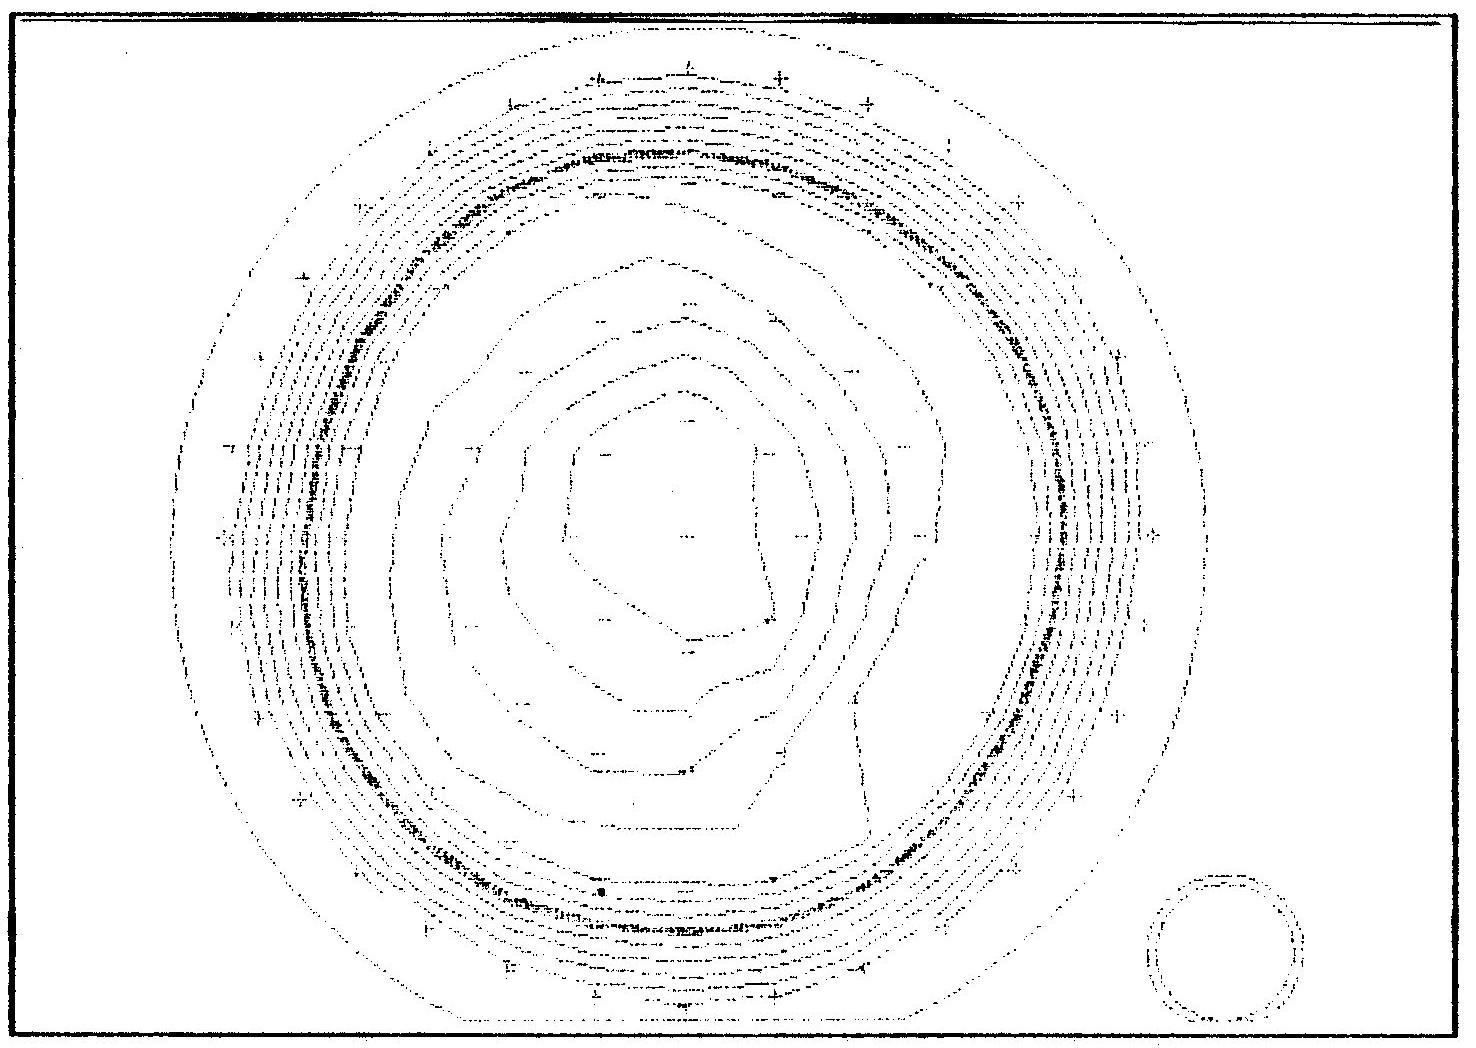
\includegraphics{Figures/fig-7-1.eps}% chktex-file 8
    \end{center}
  \caption[Area distribution of surface specific resistance of silicon
    wafer No.16]{Surface Specific Resistivity Distribution specific
    resistivity of silicon wafer No.16.}\label{fig:7.1}
  \end{minipage}
\end{figure}

\begin{figure}[h!]\centering
  \begin{minipage}[c]{\myfiguresize}
    \begin{center}
      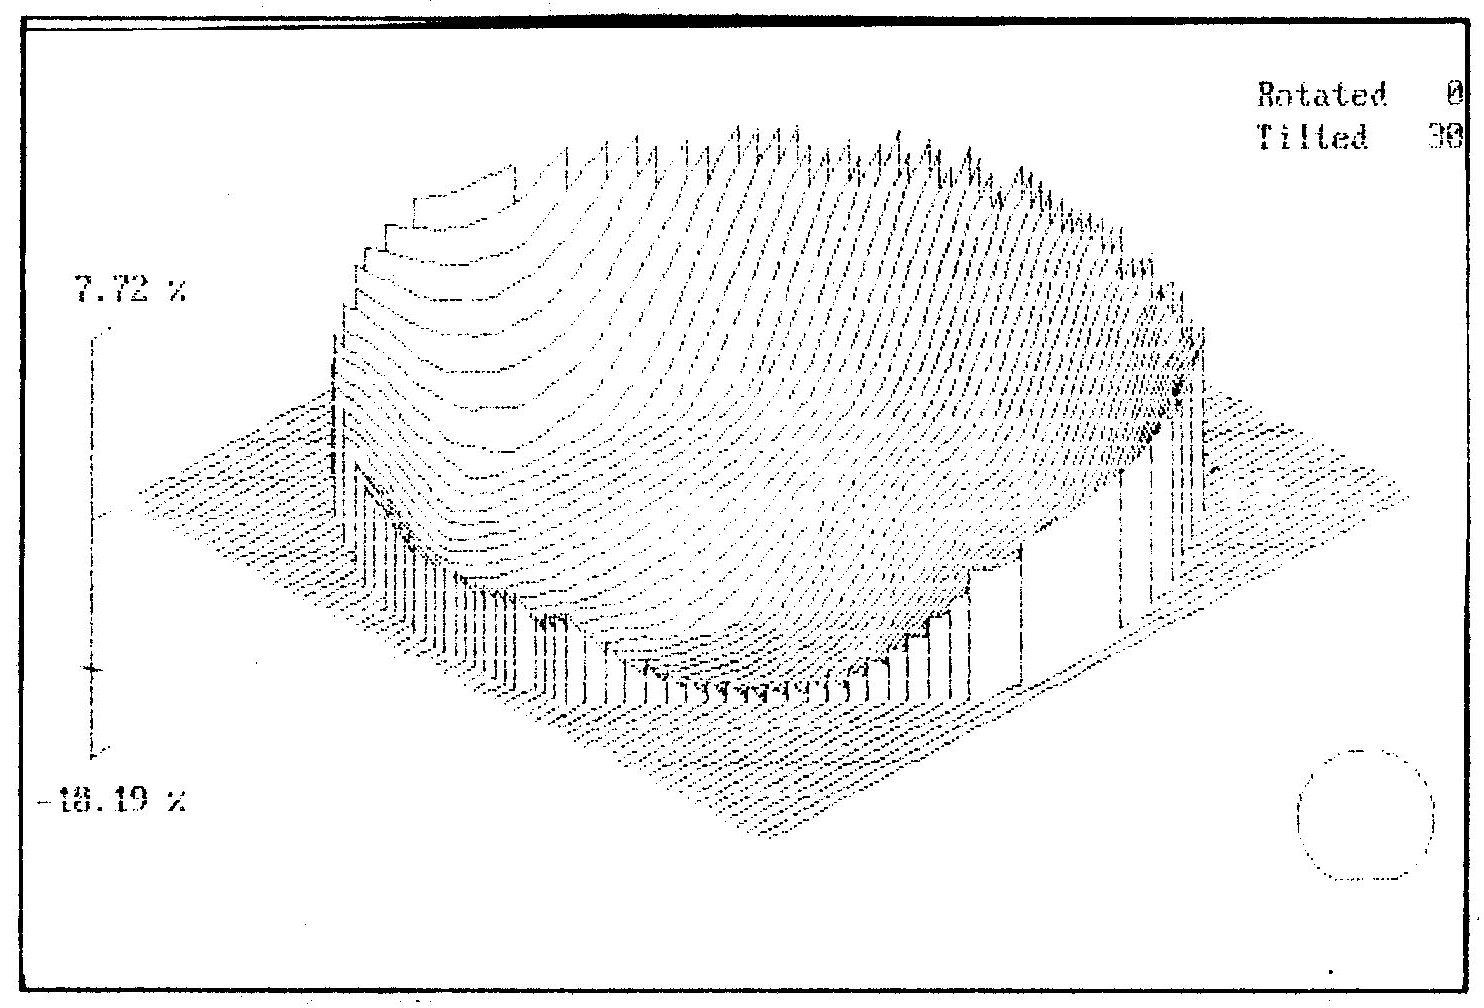
\includegraphics{Figures/fig-7-2.eps}
    \end{center}
  \caption[Area distribution of surface specific resistance of silicon
    wafer No.16]{Surface Specific Resistivity Distribution of silicon
    wafer No.16.}\label{fig:7.2}
  \end{minipage}
\end{figure}

\newpage
\begin{figure}[h!]\centering
  \begin{minipage}[c]{\myfiguresize}
    \begin{center}
      % GNUPLOT: LaTeX picture with Postscript
\begingroup
  \makeatletter
  \providecommand\color[2][]{%
    \GenericError{(gnuplot) \space\space\space\@spaces}{%
      Package color not loaded in conjunction with
      terminal option `colourtext'%
    }{See the gnuplot documentation for explanation.%
    }{Either use 'blacktext' in gnuplot or load the package
      color.sty in LaTeX.}%
    \renewcommand\color[2][]{}%
  }%
  \providecommand\includegraphics[2][]{%
    \GenericError{(gnuplot) \space\space\space\@spaces}{%
      Package graphicx or graphics not loaded%
    }{See the gnuplot documentation for explanation.%
    }{The gnuplot epslatex terminal needs graphicx.sty or graphics.sty.}%
    \renewcommand\includegraphics[2][]{}%
  }%
  \providecommand\rotatebox[2]{#2}%
  \@ifundefined{ifGPcolor}{%
    \newif\ifGPcolor
    \GPcolortrue
  }{}%
  \@ifundefined{ifGPblacktext}{%
    \newif\ifGPblacktext
    \GPblacktexttrue
  }{}%
  % define a \g@addto@macro without @ in the name:
  \let\gplgaddtomacro\g@addto@macro
  % define empty templates for all commands taking text:
  \gdef\gplbacktext{}%
  \gdef\gplfronttext{}%
  \makeatother
  \ifGPblacktext
    % no textcolor at all
    \def\colorrgb#1{}%
    \def\colorgray#1{}%
  \else
    % gray or color?
    \ifGPcolor
      \def\colorrgb#1{\color[rgb]{#1}}%
      \def\colorgray#1{\color[gray]{#1}}%
      \expandafter\def\csname LTw\endcsname{\color{white}}%
      \expandafter\def\csname LTb\endcsname{\color{black}}%
      \expandafter\def\csname LTa\endcsname{\color{black}}%
      \expandafter\def\csname LT0\endcsname{\color[rgb]{1,0,0}}%
      \expandafter\def\csname LT1\endcsname{\color[rgb]{0,1,0}}%
      \expandafter\def\csname LT2\endcsname{\color[rgb]{0,0,1}}%
      \expandafter\def\csname LT3\endcsname{\color[rgb]{1,0,1}}%
      \expandafter\def\csname LT4\endcsname{\color[rgb]{0,1,1}}%
      \expandafter\def\csname LT5\endcsname{\color[rgb]{1,1,0}}%
      \expandafter\def\csname LT6\endcsname{\color[rgb]{0,0,0}}%
      \expandafter\def\csname LT7\endcsname{\color[rgb]{1,0.3,0}}%
      \expandafter\def\csname LT8\endcsname{\color[rgb]{0.5,0.5,0.5}}%
    \else
      % gray
      \def\colorrgb#1{\color{black}}%
      \def\colorgray#1{\color[gray]{#1}}%
      \expandafter\def\csname LTw\endcsname{\color{white}}%
      \expandafter\def\csname LTb\endcsname{\color{black}}%
      \expandafter\def\csname LTa\endcsname{\color{black}}%
      \expandafter\def\csname LT0\endcsname{\color{black}}%
      \expandafter\def\csname LT1\endcsname{\color{black}}%
      \expandafter\def\csname LT2\endcsname{\color{black}}%
      \expandafter\def\csname LT3\endcsname{\color{black}}%
      \expandafter\def\csname LT4\endcsname{\color{black}}%
      \expandafter\def\csname LT5\endcsname{\color{black}}%
      \expandafter\def\csname LT6\endcsname{\color{black}}%
      \expandafter\def\csname LT7\endcsname{\color{black}}%
      \expandafter\def\csname LT8\endcsname{\color{black}}%
    \fi
  \fi
    \setlength{\unitlength}{0.0500bp}%
    \ifx\gptboxheight\undefined%
      \newlength{\gptboxheight}%
      \newlength{\gptboxwidth}%
      \newsavebox{\gptboxtext}%
    \fi%
    \setlength{\fboxrule}{0.5pt}%
    \setlength{\fboxsep}{1pt}%
\begin{picture}(7920.00,5616.00)%
    \gplgaddtomacro\gplbacktext{%
      \csname LTb\endcsname%%
      \put(1100,640){\makebox(0,0)[r]{\strut{}$1\times10^{21}$}}%
      \put(1100,2261){\makebox(0,0)[r]{\strut{}$1\times10^{22}$}}%
      \put(1100,3882){\makebox(0,0)[r]{\strut{}$1\times10^{23}$}}%
      \put(1220,440){\makebox(0,0){\strut{}$0$}}%
      \put(2012,440){\makebox(0,0){\strut{}$0.1$}}%
      \put(2805,440){\makebox(0,0){\strut{}$0.2$}}%
      \put(3597,440){\makebox(0,0){\strut{}$0.3$}}%
      \put(4390,440){\makebox(0,0){\strut{}$0.4$}}%
      \put(5182,440){\makebox(0,0){\strut{}$0.5$}}%
      \put(5974,440){\makebox(0,0){\strut{}$0.6$}}%
      \put(6767,440){\makebox(0,0){\strut{}$0.7$}}%
      \put(7559,440){\makebox(0,0){\strut{}$0.8$}}%
    }%
    \gplgaddtomacro\gplfronttext{%
      \csname LTb\endcsname%%
      \put(190,2827){\rotatebox{-270}{\makebox(0,0){\strut{}Concentration $[{m}^{-3}]$}}}%
      \put(4389,140){\makebox(0,0){\strut{}Depth $[\mu{m}]$}}%
      \put(4389,5315){\makebox(0,0){\strut{}Dopant profile}}%
    }%
    \gplbacktext
    \put(0,0){\includegraphics{/export/scratch/vbotka-thesis/Plot/Figures/fig-7-3-en}}%
    \gplfronttext
  \end{picture}%
\endgroup

    \end{center}
    \caption[Depth profile of tangents]{Depth profile of the
      interfering impurities in the subsurface region of the
      semiconductor formed by ion implantation with doses of $0.6,
      1.0, 2.0, 4.0, 5.0, 6.0, 7.0, 8.0, 20.0, 60.0 \times 10^{15}
      m^{-2}$. Shown are the $N(x)$ curves represent the mean of the
      curves measured at 304 MOS structures of each silicon
      wafer.}\label{fig:7.3}
  \end{minipage}
\end{figure}
% OBR27.BIT

\newpage
\begin{figure}[h!]
  \begin{minipage}[c]{\myfiguresize}
    \begin{center}
      % GNUPLOT: LaTeX picture with Postscript
\begingroup
  \makeatletter
  \providecommand\color[2][]{%
    \GenericError{(gnuplot) \space\space\space\@spaces}{%
      Package color not loaded in conjunction with
      terminal option `colourtext'%
    }{See the gnuplot documentation for explanation.%
    }{Either use 'blacktext' in gnuplot or load the package
      color.sty in LaTeX.}%
    \renewcommand\color[2][]{}%
  }%
  \providecommand\includegraphics[2][]{%
    \GenericError{(gnuplot) \space\space\space\@spaces}{%
      Package graphicx or graphics not loaded%
    }{See the gnuplot documentation for explanation.%
    }{The gnuplot epslatex terminal needs graphicx.sty or graphics.sty.}%
    \renewcommand\includegraphics[2][]{}%
  }%
  \providecommand\rotatebox[2]{#2}%
  \@ifundefined{ifGPcolor}{%
    \newif\ifGPcolor
    \GPcolortrue
  }{}%
  \@ifundefined{ifGPblacktext}{%
    \newif\ifGPblacktext
    \GPblacktexttrue
  }{}%
  % define a \g@addto@macro without @ in the name:
  \let\gplgaddtomacro\g@addto@macro
  % define empty templates for all commands taking text:
  \gdef\gplbacktext{}%
  \gdef\gplfronttext{}%
  \makeatother
  \ifGPblacktext
    % no textcolor at all
    \def\colorrgb#1{}%
    \def\colorgray#1{}%
  \else
    % gray or color?
    \ifGPcolor
      \def\colorrgb#1{\color[rgb]{#1}}%
      \def\colorgray#1{\color[gray]{#1}}%
      \expandafter\def\csname LTw\endcsname{\color{white}}%
      \expandafter\def\csname LTb\endcsname{\color{black}}%
      \expandafter\def\csname LTa\endcsname{\color{black}}%
      \expandafter\def\csname LT0\endcsname{\color[rgb]{1,0,0}}%
      \expandafter\def\csname LT1\endcsname{\color[rgb]{0,1,0}}%
      \expandafter\def\csname LT2\endcsname{\color[rgb]{0,0,1}}%
      \expandafter\def\csname LT3\endcsname{\color[rgb]{1,0,1}}%
      \expandafter\def\csname LT4\endcsname{\color[rgb]{0,1,1}}%
      \expandafter\def\csname LT5\endcsname{\color[rgb]{1,1,0}}%
      \expandafter\def\csname LT6\endcsname{\color[rgb]{0,0,0}}%
      \expandafter\def\csname LT7\endcsname{\color[rgb]{1,0.3,0}}%
      \expandafter\def\csname LT8\endcsname{\color[rgb]{0.5,0.5,0.5}}%
    \else
      % gray
      \def\colorrgb#1{\color{black}}%
      \def\colorgray#1{\color[gray]{#1}}%
      \expandafter\def\csname LTw\endcsname{\color{white}}%
      \expandafter\def\csname LTb\endcsname{\color{black}}%
      \expandafter\def\csname LTa\endcsname{\color{black}}%
      \expandafter\def\csname LT0\endcsname{\color{black}}%
      \expandafter\def\csname LT1\endcsname{\color{black}}%
      \expandafter\def\csname LT2\endcsname{\color{black}}%
      \expandafter\def\csname LT3\endcsname{\color{black}}%
      \expandafter\def\csname LT4\endcsname{\color{black}}%
      \expandafter\def\csname LT5\endcsname{\color{black}}%
      \expandafter\def\csname LT6\endcsname{\color{black}}%
      \expandafter\def\csname LT7\endcsname{\color{black}}%
      \expandafter\def\csname LT8\endcsname{\color{black}}%
    \fi
  \fi
    \setlength{\unitlength}{0.0500bp}%
    \ifx\gptboxheight\undefined%
      \newlength{\gptboxheight}%
      \newlength{\gptboxwidth}%
      \newsavebox{\gptboxtext}%
    \fi%
    \setlength{\fboxrule}{0.5pt}%
    \setlength{\fboxsep}{1pt}%
\begin{picture}(7920.00,5616.00)%
    \gplgaddtomacro\gplbacktext{%
      \csname LTb\endcsname%%
      \put(740,640){\makebox(0,0)[r]{\strut{}$0.1$}}%
      \put(740,2215){\makebox(0,0)[r]{\strut{}$1$}}%
      \put(740,3790){\makebox(0,0)[r]{\strut{}$10$}}%
      \put(860,440){\makebox(0,0){\strut{}$0.1$}}%
      \put(3168,440){\makebox(0,0){\strut{}$1$}}%
      \put(5475,440){\makebox(0,0){\strut{}$10$}}%
    }%
    \gplgaddtomacro\gplfronttext{%
      \csname LTb\endcsname%%
      \put(190,2827){\rotatebox{-270}{\makebox(0,0){\strut{}Activated ions ${10}^{15}[{m}^{-2}]$}}}%
      \put(4209,140){\makebox(0,0){\strut{}Implant Dose $D_{i}{10}^{15}[{m}^{-2}]$}}%
      \put(4209,5315){\makebox(0,0){\strut{}Dopant activation}}%
    }%
    \gplgaddtomacro\gplbacktext{%
      \csname LTb\endcsname%%
      \put(740,640){\makebox(0,0)[r]{\strut{}$0.1$}}%
      \put(740,2215){\makebox(0,0)[r]{\strut{}$1$}}%
      \put(740,3790){\makebox(0,0)[r]{\strut{}$10$}}%
      \put(860,440){\makebox(0,0){\strut{}$0.1$}}%
      \put(3168,440){\makebox(0,0){\strut{}$1$}}%
      \put(5475,440){\makebox(0,0){\strut{}$10$}}%
    }%
    \gplgaddtomacro\gplfronttext{%
      \csname LTb\endcsname%%
      \put(190,2827){\rotatebox{-270}{\makebox(0,0){\strut{}Activated ions ${10}^{15}[{m}^{-2}]$}}}%
      \put(4209,140){\makebox(0,0){\strut{}Implant Dose $D_{i}{10}^{15}[{m}^{-2}]$}}%
      \put(4209,5315){\makebox(0,0){\strut{}Dopant activation}}%
    }%
    \gplbacktext
    \put(0,0){\includegraphics{/export/scratch/vbotka-thesis/Plot/Figures/fig-7-4-en}}%
    \gplfronttext
  \end{picture}%
\endgroup

    \end{center}
    \caption[Dependence of mean value of activated ions
      $\overline{D}=E(\int(N(x)-N_{b})dx)$ on the implanted ion dose
      $D_{i}$] {Dependence of mean value of activated ions
      $\overline{D}=E(\int(N(x)-N_{b})dx)$ on the implanted ion dose
      $D_{i}$. Data from Table~\ref{tab:7.2}}\label{fig:7.4}
  \end{minipage}
\end{figure}
%OBR29.BIT

Table~\ref{tab:7.2} contains the values of the implant dose entered
during the implantation process $D_{i}$, the mean value $\overline D$
and the standard deviation of $\delta D$ of the activated ions
measured by the procedure described in section~\ref{sec:6.1}.
 
\begin{table}[h!]\centering
  \begin{minipage}[c]{\myfiguresize}
    \begin{center}
      \begin{tabular}{c c c c}
        No. & ${D_{i}}{10}^{15}[m^{-2}]$ & $\overline{D}{10}^{15}[m^{-2}]$ & $\delta{D}{10}^{15}[m^{-2}]$\\
        \hline
        1 & 0.6 & 0.39 & 0.02\\
        3 & 1.0 & 0.59 & 0.08\\
        5 & 2.0 & 1.20 & 0.06\\
        7 & 4.0 & 2.67 & 0.09\\
        9 & 5.0 & 3.40 & 0.13\\
        11 & 6.0 & 4.07 & 0.13\\
        13 & 7.0 & 4.72 & 0.14\\
        15 & 8.0 & 5.49 & 0.09\\
        17 & 20.0 & 14.41 & 0.35\\
        19 & 60.0 & 42.63 & 0.21\\
      \end{tabular}
    \end{center}
    \caption[Implantation dose $D_{i}$]{Implantation dose $D_{i}$, the
      calculated mean value of the implanted and activated ions in the
      semiconductor $\overline D$ and its standard deviation $\delta
      D$ on the silicon wafer.}\label{tab:7.2}
  \end{minipage}
\end{table}

To check the reproducibility of the implantation process, the
concentration profiles on 3 additional silicon wafers were
measured. In the Table~\ref{tab:7.3} are the implantation dose values
for the three pairs of silicon wafers that were implanted with the
same dose.

\begin{table}[h!]\centering
  \begin{minipage}[c]{\myfiguresize}
    \begin{center}
      \begin{tabular}{c c c c}
        No. & $D_{i} 10^{15} [m^{-2}]$ & $\overline D 10^{15} [m^{-2}]$ & $\delta D 10^{15} [m^{-2}]$\\
        \hline
        9 & 5.0 & 3.40 & 0.13\\
        10 & 5.0 & 3.56 & 0.06\\
        11 & 6.0 & 4.07 & 0.13\\
        12 & 6.0 & 4.03 & 0.12\\
        15 & 8.0 & 5.49 & 0.09\\
        16 & 8.0 & 5.46 & 0.08\\
      \end{tabular}
    \end{center}
    \caption[Implantation dose $D_{i}$]{Implantation dose $D_{i}$, the
      calculated mean of the dose of implanted and activated ions in
      the semiconductor $\overline D$ and its standard deviation
      $\delta D$ on the silicon wafer.}\label{tab:7.3}
  \end{minipage}
\end{table}

As can be seen from Tables~\ref{tab:7.2} and~\ref{tab:7.3}, the
measured dose of activated ions is always less than the dose entered
in the process of implantation. This is partly due to the implanted
ions trapped in the oxide layer and partly due to incomplete
activation of the implanted ions in the semiconductor. In order to
evaluate the dependence between the implanted and measured dose, we
used linear regression to calculate the coefficient $b$

\begin{equation}\label{eq:7.1}
  \overline D = bD_{i}
\end{equation}

which had the value of $b = 0.71$. We also plotted the dependence
$\overline D = f(D_{i})$ in Figure~\ref{fig:7.4}.

We found out that $71\%$ from the implanted ions became electrically
active. To determine the degree of dependence between the implanted
dose and the amount of electrically active impurities in the
semiconductor, which were implanted, we calculated the correlation
coefficient between these quantities. We used the relationship

\begin{equation}\label{eq:7.2}
  R(X,Y) = \frac{E([X-E(X)][Y-E(Y)])}{D(X)D(Y)}
\end{equation}

, which is given for example in~\cite{7.1}. In the
equation~\ref{eq:7.2} X and Y represent random variables, E represents
the mean and D denotes the standard deviation. This way we have
obtained the value of the correlation coefficient

\centerline{$R(D_{i}, \overline{D}) = 0.99$}

taking the values of $D_{i}$ and $\overline{D}$ as realizations of the
random variable and we used all the values given in
Table~\ref{tab:7.2} and~\ref{tab:7.3}. It may be noted that in the
theory of probability the theorem is proved that $\rvert R(X,Y)\rvert
= 1$ precisely if, with probability 1, is valid

\centerline{$Y = a + b X$}

It follows that the dependence between the values of $D_{i}$ and
$\overline D$ is linear in this case.

Using a professional program, purchased by Tesla Piešťany, to
simulate the process of ion implantation, the curves were
calculated of impurity concentration for doses of 0.6, 5.0 and 60.0
$\times10^{15}m^{-2}$.  The concentration profile curves were
simulated based on the specified implantation conditions using the
Pearson IV\@ method.  A comparison of the measured and simulated
impurity concentration curves is shown in Figure~\ref{fig:7.5}.

\begin{figure}[h!]\centering
  \begin{minipage}[c]{\myfiguresize}
    \begin{center}
      % GNUPLOT: LaTeX picture with Postscript
\begingroup
  \makeatletter
  \providecommand\color[2][]{%
    \GenericError{(gnuplot) \space\space\space\@spaces}{%
      Package color not loaded in conjunction with
      terminal option `colourtext'%
    }{See the gnuplot documentation for explanation.%
    }{Either use 'blacktext' in gnuplot or load the package
      color.sty in LaTeX.}%
    \renewcommand\color[2][]{}%
  }%
  \providecommand\includegraphics[2][]{%
    \GenericError{(gnuplot) \space\space\space\@spaces}{%
      Package graphicx or graphics not loaded%
    }{See the gnuplot documentation for explanation.%
    }{The gnuplot epslatex terminal needs graphicx.sty or graphics.sty.}%
    \renewcommand\includegraphics[2][]{}%
  }%
  \providecommand\rotatebox[2]{#2}%
  \@ifundefined{ifGPcolor}{%
    \newif\ifGPcolor
    \GPcolortrue
  }{}%
  \@ifundefined{ifGPblacktext}{%
    \newif\ifGPblacktext
    \GPblacktexttrue
  }{}%
  % define a \g@addto@macro without @ in the name:
  \let\gplgaddtomacro\g@addto@macro
  % define empty templates for all commands taking text:
  \gdef\gplbacktext{}%
  \gdef\gplfronttext{}%
  \makeatother
  \ifGPblacktext
    % no textcolor at all
    \def\colorrgb#1{}%
    \def\colorgray#1{}%
  \else
    % gray or color?
    \ifGPcolor
      \def\colorrgb#1{\color[rgb]{#1}}%
      \def\colorgray#1{\color[gray]{#1}}%
      \expandafter\def\csname LTw\endcsname{\color{white}}%
      \expandafter\def\csname LTb\endcsname{\color{black}}%
      \expandafter\def\csname LTa\endcsname{\color{black}}%
      \expandafter\def\csname LT0\endcsname{\color[rgb]{1,0,0}}%
      \expandafter\def\csname LT1\endcsname{\color[rgb]{0,1,0}}%
      \expandafter\def\csname LT2\endcsname{\color[rgb]{0,0,1}}%
      \expandafter\def\csname LT3\endcsname{\color[rgb]{1,0,1}}%
      \expandafter\def\csname LT4\endcsname{\color[rgb]{0,1,1}}%
      \expandafter\def\csname LT5\endcsname{\color[rgb]{1,1,0}}%
      \expandafter\def\csname LT6\endcsname{\color[rgb]{0,0,0}}%
      \expandafter\def\csname LT7\endcsname{\color[rgb]{1,0.3,0}}%
      \expandafter\def\csname LT8\endcsname{\color[rgb]{0.5,0.5,0.5}}%
    \else
      % gray
      \def\colorrgb#1{\color{black}}%
      \def\colorgray#1{\color[gray]{#1}}%
      \expandafter\def\csname LTw\endcsname{\color{white}}%
      \expandafter\def\csname LTb\endcsname{\color{black}}%
      \expandafter\def\csname LTa\endcsname{\color{black}}%
      \expandafter\def\csname LT0\endcsname{\color{black}}%
      \expandafter\def\csname LT1\endcsname{\color{black}}%
      \expandafter\def\csname LT2\endcsname{\color{black}}%
      \expandafter\def\csname LT3\endcsname{\color{black}}%
      \expandafter\def\csname LT4\endcsname{\color{black}}%
      \expandafter\def\csname LT5\endcsname{\color{black}}%
      \expandafter\def\csname LT6\endcsname{\color{black}}%
      \expandafter\def\csname LT7\endcsname{\color{black}}%
      \expandafter\def\csname LT8\endcsname{\color{black}}%
    \fi
  \fi
    \setlength{\unitlength}{0.0500bp}%
    \ifx\gptboxheight\undefined%
      \newlength{\gptboxheight}%
      \newlength{\gptboxwidth}%
      \newsavebox{\gptboxtext}%
    \fi%
    \setlength{\fboxrule}{0.5pt}%
    \setlength{\fboxsep}{1pt}%
\begin{picture}(7920.00,5616.00)%
    \gplgaddtomacro\gplbacktext{%
      \csname LTb\endcsname%%
      \put(1100,640){\makebox(0,0)[r]{\strut{}$1\times10^{21}$}}%
      \put(1100,2261){\makebox(0,0)[r]{\strut{}$1\times10^{22}$}}%
      \put(1100,3882){\makebox(0,0)[r]{\strut{}$1\times10^{23}$}}%
      \put(1220,440){\makebox(0,0){\strut{}$0$}}%
      \put(2012,440){\makebox(0,0){\strut{}$0.1$}}%
      \put(2805,440){\makebox(0,0){\strut{}$0.2$}}%
      \put(3597,440){\makebox(0,0){\strut{}$0.3$}}%
      \put(4390,440){\makebox(0,0){\strut{}$0.4$}}%
      \put(5182,440){\makebox(0,0){\strut{}$0.5$}}%
      \put(5974,440){\makebox(0,0){\strut{}$0.6$}}%
      \put(6767,440){\makebox(0,0){\strut{}$0.7$}}%
      \put(7559,440){\makebox(0,0){\strut{}$0.8$}}%
    }%
    \gplgaddtomacro\gplfronttext{%
      \csname LTb\endcsname%%
      \put(190,2827){\rotatebox{-270}{\makebox(0,0){\strut{}Concentration $[{m}^{-3}]$}}}%
      \put(4389,140){\makebox(0,0){\strut{}Depth $[\mu{m}]$}}%
      \put(4389,5315){\makebox(0,0){\strut{}Comparison of measured vs. simulated dopant profiles.}}%
    }%
    \gplbacktext
    \put(0,0){\includegraphics{/export/scratch/vbotka-thesis/Plot/Figures/fig-7-5-en}}%
    \gplfronttext
  \end{picture}%
\endgroup

    \end{center}
    \caption[Comparison of the mean values of the measured curves
      $N(x)$ and simulated using the Pearson IV method]{Comparison of
      means values of the measured $N(x)$ and simulated $N(x)$ curves
      Pearson IV for doses $0.6, 5.0, 60.0 \times 10^{15} m^{-2}$. The
      measured values show lower concentration.}\label{fig:7.5}
  \end{minipage}
\end{figure}
% OBR33.BIT

In the process of calculating the depth profiles of the intervening
admixtures, we simultaneously also determined the values of the
stresses of the aligned bands $V_{fb}$ for each MOS\@ structure
tested. Using a separate program that determines based on the data
contained in a given data file, the mean value and standard deviation
of the stored parameters, we calculated the mean of $\overline V{fb}$
and the standard deviation of $\delta V{fb}$. At the same time, using
the same procedure, we determined the values of $\overline h_{ox}$ and
$\delta h_{ox}$, which are for each silicon slabs are given in
Table~\ref{tab:7.4}.

It can be seen from the table~\ref{tab:7.4} that the values of
$\overline V_{fb}$ are related to the mean values of the oxide layer
thickness $\overline h_{ox}$, so we have shown this dependence in
Figure~\ref{fig:7.6}.

\newpage
\begin{figure}[h!]
  \begin{minipage}[c]{\myfiguresize}
    \begin{center}
      % GNUPLOT: LaTeX picture with Postscript
\begingroup
  \makeatletter
  \providecommand\color[2][]{%
    \GenericError{(gnuplot) \space\space\space\@spaces}{%
      Package color not loaded in conjunction with
      terminal option `colourtext'%
    }{See the gnuplot documentation for explanation.%
    }{Either use 'blacktext' in gnuplot or load the package
      color.sty in LaTeX.}%
    \renewcommand\color[2][]{}%
  }%
  \providecommand\includegraphics[2][]{%
    \GenericError{(gnuplot) \space\space\space\@spaces}{%
      Package graphicx or graphics not loaded%
    }{See the gnuplot documentation for explanation.%
    }{The gnuplot epslatex terminal needs graphicx.sty or graphics.sty.}%
    \renewcommand\includegraphics[2][]{}%
  }%
  \providecommand\rotatebox[2]{#2}%
  \@ifundefined{ifGPcolor}{%
    \newif\ifGPcolor
    \GPcolortrue
  }{}%
  \@ifundefined{ifGPblacktext}{%
    \newif\ifGPblacktext
    \GPblacktexttrue
  }{}%
  % define a \g@addto@macro without @ in the name:
  \let\gplgaddtomacro\g@addto@macro
  % define empty templates for all commands taking text:
  \gdef\gplbacktext{}%
  \gdef\gplfronttext{}%
  \makeatother
  \ifGPblacktext
    % no textcolor at all
    \def\colorrgb#1{}%
    \def\colorgray#1{}%
  \else
    % gray or color?
    \ifGPcolor
      \def\colorrgb#1{\color[rgb]{#1}}%
      \def\colorgray#1{\color[gray]{#1}}%
      \expandafter\def\csname LTw\endcsname{\color{white}}%
      \expandafter\def\csname LTb\endcsname{\color{black}}%
      \expandafter\def\csname LTa\endcsname{\color{black}}%
      \expandafter\def\csname LT0\endcsname{\color[rgb]{1,0,0}}%
      \expandafter\def\csname LT1\endcsname{\color[rgb]{0,1,0}}%
      \expandafter\def\csname LT2\endcsname{\color[rgb]{0,0,1}}%
      \expandafter\def\csname LT3\endcsname{\color[rgb]{1,0,1}}%
      \expandafter\def\csname LT4\endcsname{\color[rgb]{0,1,1}}%
      \expandafter\def\csname LT5\endcsname{\color[rgb]{1,1,0}}%
      \expandafter\def\csname LT6\endcsname{\color[rgb]{0,0,0}}%
      \expandafter\def\csname LT7\endcsname{\color[rgb]{1,0.3,0}}%
      \expandafter\def\csname LT8\endcsname{\color[rgb]{0.5,0.5,0.5}}%
    \else
      % gray
      \def\colorrgb#1{\color{black}}%
      \def\colorgray#1{\color[gray]{#1}}%
      \expandafter\def\csname LTw\endcsname{\color{white}}%
      \expandafter\def\csname LTb\endcsname{\color{black}}%
      \expandafter\def\csname LTa\endcsname{\color{black}}%
      \expandafter\def\csname LT0\endcsname{\color{black}}%
      \expandafter\def\csname LT1\endcsname{\color{black}}%
      \expandafter\def\csname LT2\endcsname{\color{black}}%
      \expandafter\def\csname LT3\endcsname{\color{black}}%
      \expandafter\def\csname LT4\endcsname{\color{black}}%
      \expandafter\def\csname LT5\endcsname{\color{black}}%
      \expandafter\def\csname LT6\endcsname{\color{black}}%
      \expandafter\def\csname LT7\endcsname{\color{black}}%
      \expandafter\def\csname LT8\endcsname{\color{black}}%
    \fi
  \fi
    \setlength{\unitlength}{0.0500bp}%
    \ifx\gptboxheight\undefined%
      \newlength{\gptboxheight}%
      \newlength{\gptboxwidth}%
      \newsavebox{\gptboxtext}%
    \fi%
    \setlength{\fboxrule}{0.5pt}%
    \setlength{\fboxsep}{1pt}%
\begin{picture}(7920.00,5616.00)%
    \gplgaddtomacro\gplbacktext{%
      \csname LTb\endcsname%%
      \put(860,640){\makebox(0,0)[r]{\strut{}$-1.7$}}%
      \put(860,1369){\makebox(0,0)[r]{\strut{}$-1.6$}}%
      \put(860,2098){\makebox(0,0)[r]{\strut{}$-1.5$}}%
      \put(860,2828){\makebox(0,0)[r]{\strut{}$-1.4$}}%
      \put(860,3557){\makebox(0,0)[r]{\strut{}$-1.3$}}%
      \put(860,4286){\makebox(0,0)[r]{\strut{}$-1.2$}}%
      \put(860,5015){\makebox(0,0)[r]{\strut{}$-1.1$}}%
      \put(980,440){\makebox(0,0){\strut{}$92$}}%
      \put(1992,440){\makebox(0,0){\strut{}$94$}}%
      \put(3004,440){\makebox(0,0){\strut{}$96$}}%
      \put(4016,440){\makebox(0,0){\strut{}$98$}}%
      \put(5029,440){\makebox(0,0){\strut{}$100$}}%
      \put(6041,440){\makebox(0,0){\strut{}$102$}}%
      \put(7053,440){\makebox(0,0){\strut{}$104$}}%
    }%
    \gplgaddtomacro\gplfronttext{%
      \csname LTb\endcsname%%
      \put(190,2827){\rotatebox{-270}{\makebox(0,0){\strut{}Flatband Voltage $[V]$}}}%
      \put(4269,140){\makebox(0,0){\strut{}Oxide thickness $[nm]$}}%
      \put(4269,5315){\makebox(0,0){\strut{}Flatband voltage / Oxide thickness}}%
    }%
    \gplbacktext
    \put(0,0){\includegraphics{/export/scratch/vbotka-thesis/Plot/Figures/fig-7-6-en}}%
    \gplfronttext
  \end{picture}%
\endgroup

    \end{center}
    \caption[Dependence of the mean value of $\overline V_{fb}$ on the
      mean value of the oxide layer thickness $\overline
      h_{ox}$]{Dependence of the mean value of the flatband voltage
      $\overline V_{fb}$ on the mean value of the thickness of the
      oxide layer $\overline h_{ox}$ for silicon wafers number 1, 3,
      5, 7, 9, 11, 13, 15 and 17. Data from
      Table~\ref{tab:7.4}}\label{fig:7.6}
  \end{minipage}
\end{figure}

\begin{table}[h!]\centering
  \begin{minipage}[c]{\myfiguresize}
    \begin{center}
      \begin{tabular}{c c c c c}
        No. & $\overline V_{fb} [V]$ & $\delta V_{fb} [V]$ & $\overline h_{ox} [nm]$ & $\delta h_{ox} [nm]$\\
        \hline
        1 & -1.24 & 0.07 & 94.14 & 0.89\\
        3 & -1.43 & 0.07 & 97.79 & 0.80\\
        5 & -1.35 & 0.08 & 97.26 & 0.28\\
        7 & -1.40 & 0.09 & 98.15 & 0.35\\
        9 & -1.52 & 0.09 & 102.85 & 0.53\\
        11 & -1.48 & 0.08 & 101.65 & 0.32\\
        13 & -1.38 & 0.08 & 100.94 & 0.41\\
        15 & -1.33 & 0.07 & 100.80 & 0.16\\
        17 & -1.59 & 0.08 & 99.93 & 0.22\\
        19 & -2.43 & 0.16 & 99.67 & 0.19\\
      \end{tabular}
    \end{center}
    \caption[Mean and standard deviation of the flat-band voltage and
      the thickness of the oxide]{Mean and standard deviation of the
      flat-band voltage and the thickness of the
      oxide.}\label{tab:7.4}
  \end{minipage}
\end{table}

Correlation coefficient value

\centerline{$R(\overline V_{fb} ,\overline h_{ox}) = -0.78$}

agrees with the theoretical relationship defining the dependence of
$V_{fb}$ on the magnitude of the breakdown charge in the oxide layer
and at the interface $Si-SiO_{2}$ $Q_{dc}$ and on the magnitude of the
oxide layer capacitance $C_{ox}$

\begin{equation}\label{eq:7.3}
  V_{fb}  = \varphi_{ms} + \frac{Q_{dc}}{C_{ox}}
\end{equation}

where $\varphi_{ms}$ represents the difference in output potentials
between the semiconductor and the metal. For linear regression
coefficients

\centerline{$V_{fb}  = a + b h_{ox}$}

we obtained the values

\centerline{$a = 5.48 \times 10^{-3} \qquad b = -1.41 \times 10^{7}$}

The interface trap density was determined on four silicon wafers
$Si-SiO_2$ $D_{it}$. As can be seen from Table~\ref{tab:7.5}, the mean
values of $\overline D_{it}$ are in the region of $2.0-5.0\times
10^{14}$, which speaks for the good quality of the $Si-SiO_{2}$
interface. The crystal quality is indicated by the magnitude of the
generation time of the minority charge carriers. In order to compare
the quality of the crystal for individual slabs, we determined on each
silicon slab the area distribution of $³tau_{g}$ at depths ranging
from $0.9$ to $1.3 m$. For all slabs we then determined the mean value
of $\overline\tau_{g}$ and the standard deviation of
$\overline\tau_{g}$ deviation of $\delta\tau_{g}$, the values of which
are given in Table~\ref{tab:7.6}. The values of $\overline\tau_{g}$
range in between $0.41\ and\ 2.25 ms$, indicating a high quality of
the substrate. At the same time, it can be seen from
Table~\ref{tab:7.6} that the values of $\overline \tau_{g}$ are
randomly varying and cannot be found dependence on the other
previously mentioned parameters.

\begin{table}[h!]\centering
  \begin{minipage}[c]{\myfiguresize}
    \begin{center}
      \begin{tabular}{c c c}
        No. & ${\bar{D_{it}}}[m^{-2}eV^{-1}]$ & $\delta D_{it}[m^{-2}eV^{-1}]$\\
        \hline
        3 & $4.42 \times 10^{14}$ & $0.25 \times 10^{14}$\\
        7 & $2.60 \times 10^{14}$ & $0.15 \times 10^{14}$\\
        9 & $2.74 \times 10^{14}$ & $0.15 \times 10^{14}$\\
        12 & $3.55 \times 10^{14}$ & $0.16 \times 10^{14}$\\
      \end{tabular}
    \end{center}
    \caption[Mean and standard deviation of trap densities of the
      $Si-SiO_{2}$ interface at the center of the forbidden
      band.]{Mean value and standard deviation of the trap density of
      the $Si-SiO_{2}$ interface at the center of the forbidden
      band.}\label{tab:7.5}
  \end{minipage}
\end{table}

\begin{table}[h!]\centering
  \begin{minipage}[c]{\myfiguresize}
    \begin{center}
      \begin{tabular}{c c c}
        No. & ${\bar{\tau_{g}}}[ms]$ & $\delta\tau_{g}[ms]$\\
        \hline
        1 & 1.93 & 0.12\\
        3 & 1.48 & 0.09\\
        5 & 1.84 & 0.09\\
        7 & 1.67 & 0.10\\
        10 & 1.95 & 0.09\\
        12 & 0.41 & 0.02\\
        15 & 1.74 & 0.09\\
        17 & 2.25 & 0.14\\
      \end{tabular}
    \end{center}
    \caption[Mean and standard deviation of generation time of life of
      minority carriers of charge]{Mean and standard deviation of the
      generational lifetime of minority carriers of
      charge.}\label{tab:7.6}
  \end{minipage}
\end{table}


\begin{thebibliography}{}
\bibitem[7.1]{7.1}
  Renyi A.: Theory of Probability. Academia Prague 1972.
\end{thebibliography}
